\documentclass{uofa-eng-assignment}
\usepackage{amsmath}
\usepackage{enumerate}% http://ctan.org/pkg/enumerate
\usepackage{lipsum}
\usepackage{hyperref}
\usepackage{amsmath, amsthm, amssymb, amsfonts, physics}
\usepackage{mathtools}
\usepackage{graphicx}
\usepackage{fdsymbol}

\hypersetup{
    colorlinks=true,
    linkcolor=blue,
    filecolor=magenta,
    urlcolor=cyan,
    pdftitle={Overleaf Example},
    pdfpagemode=FullScreen,
}

\graphicspath{ {./images/} }

\DeclareRobustCommand{\rchi}{{\mathpalette\irchi\relax}}

\newcommand{\infdiv}{D\infdivx}
\newcommand{\irchi}[2]{\raisebox{\depth}{$#1\chi$}} % inner command, used by \rchi
\newcommand\aug{\fboxsep=-\fboxrule\!\!\!\fbox{\strut}\!\!\!}
\newcommand*{\name}{\textbf{Luke Nguyen}}
\newcommand*{\id}{\textbf{D5850A}}
\newcommand*{\course}{Statistical Methods and Data Analysis (EN.625.603)}
\newcommand*{\assignment}{Midterm Exam}

\begin{document} \maketitle
%%%%%%%%%%%%%%%%%%%%%%%%%%%%%%%%%%%%%%%%%%%%%%%%%%%%%%%%%%%%%%%%%%%%%%%%%%%%%%%%%%%%%%%%%%%%%%%%%%%%    
\begin{enumerate}
    %%%%%%%%%%%%%%%%%%%%%%%%%%%%%%%%%%%%%%%%%%%%%%%%%%%%%%%%%%%%%%%%%%%%%%%%%%%%%%%%%%%%%%%%%%%%%%%%%%%%    
    %%%%%%%%%%%%%%%%%%%%%%%%%%%%%%%%%%%%%%%%%%%%%%%%%%%%%%%%%%%%%%%%%%%%%%%%%%%%%%%%%%%%%%%%%%%%%%%%%%%%    
    %%%%%%%%%%%%%%%%%%%%%%%%%%%%%%%%%%%%%%%%%%%%%%%%%%%%%%%%%%%%%%%%%%%%%%%%%%%%%%%%%%%%%%%%%%%%%%%%%%%%    
    %%%%%%%%%%%%%%%%%%%%%%%%%%%%%%%%%%%%%%%%%%%%%%%%%%%%%%%%%%%%%%%%%%%%%%%%%%%%%%%%%%%%%%%%%%%%%%%%%%%%    
    %%%%%%%%%%%%%%%%%%%%%%%%%%%%%%%%%%%%%%%%%%%%%%%%%%%%%%%%%%%%%%%%%%%%%%%%%%%%%%%%%%%%%%%%%%%%%%%%%%%%    
    \item[]
        \textbf{Question 1} \\
        Suppose that a telephone number is 534-0826. If the first 3 digits of this number are written
        down in random order and then the last 4 digits of this number are written down in random order
        in an attempt to obtain the correct telephone number, what is the probability of each of the
        following events?
        \begin{enumerate}
            \item All 7 digits are correctly placed.
            \item The first 3 digits are correctly placed and only 2 of the remaining digits are
                  incorrectly placed.
        \end{enumerate}

        \textbf{Solution}
        \begin{enumerate}
            \item Probability the first 3 digits are correctly placed is
                  \begin{align*}
                      \frac{1}{3!} = \frac{1}{6}
                  \end{align*}
                  Probability the last 4 digits are correctly placed is
                  \begin{align*}
                      \frac{1}{4!} = \frac{1}{24}
                  \end{align*}
                  We observed that the order of the first 3 digits and the last 4 digits are independent. Thus the probability of all 7 digits are correctly placed is
                  \begin{align*}
                      \frac{1}{6} \times \frac{1}{24} =  \boldsymbol{\frac{1}{144}}
                  \end{align*}
            \item The number of ways for 2 digits to be incorrectly placed is
                  \begin{align*}
                      \binom{4}{2} = 6
                  \end{align*}
                  The probability of 2 digits out of the last 4 digits are incorrectly placed is
                  \begin{align*}
                      \frac{6}{4!} = \frac{1}{4}
                  \end{align*}
                  The probability of the first 3 digits are correctly placed and only 2 of the remaining digits are incorrectly placed is
                  \begin{align*}
                      \frac{1}{6} \times \frac{1}{4} = \boldsymbol{\frac{1}{24}}
                  \end{align*}
        \end{enumerate}
        %%%%%%%%%%%%%%%%%%%%%%%%%%%%%%%%%%%%%%%%%%%%%%%%%%%%%%%%%%%%%%%%%%%%%%%%%%%%%%%%%%%%%%%%%%%%%%%%%%%%       
        %%%%%%%%%%%%%%%%%%%%%%%%%%%%%%%%%%%%%%%%%%%%%%%%%%%%%%%%%%%%%%%%%%%%%%%%%%%%%%%%%%%%%%%%%%%%%%%%%%%%       
        %%%%%%%%%%%%%%%%%%%%%%%%%%%%%%%%%%%%%%%%%%%%%%%%%%%%%%%%%%%%%%%%%%%%%%%%%%%%%%%%%%%%%%%%%%%%%%%%%%%%       
        \textbf{Question 2} \\
        Given a collection of seven people, in which three are Data Science majors and four are ACM
        majors. If a committee of three people is picked at random, what is the probability that the
        committee contains one Data Science major and two ACM majors?

        \textbf{Solution} \\
        The number of ways to pick a committee of three people from seven people where one of them is data sience major and two of them are ACM majors is
        \begin{align*}
            \binom{3}{1} \times \binom{4}{2} = 3 \times 6 = 18
        \end{align*}
        The number of ways to pick a committe of three people from seven people is
        \begin{align*}
            \binom{7}{3} = 35
        \end{align*}
        The probability that the committee contains one Data Science major and two ACM majors is
        \begin{align*}
            \frac{18}{35} = \boldsymbol{\frac{18}{35}}
        \end{align*}
        %%%%%%%%%%%%%%%%%%%%%%%%%%%%%%%%%%%%%%%%%%%%%%%%%%%%%%%%%%%%%%%%%%%%%%%%%%%%%%%%%%%%%%%%%%%%%%%%%%%%       
        %%%%%%%%%%%%%%%%%%%%%%%%%%%%%%%%%%%%%%%%%%%%%%%%%%%%%%%%%%%%%%%%%%%%%%%%%%%%%%%%%%%%%%%%%%%%%%%%%%%%       
        %%%%%%%%%%%%%%%%%%%%%%%%%%%%%%%%%%%%%%%%%%%%%%%%%%%%%%%%%%%%%%%%%%%%%%%%%%%%%%%%%%%%%%%%%%%%%%%%%%%%       
        \textbf{Question 3} \\
        Ninety percent of the disk drives manufactured by the COMDISK Company are known to
        function properly. For a collection of 18 disk drives, find the probability that at least 15 function
        properly.

        \textbf{Solution} \\
        Let $X$ be the number of disk drives that function properly. $X$ is a binomial random variable with $n = 18$ and $p = 0.9$. The probability that at least 15 function properly is
        \begin{align*}
            P(X \ge 15) & = \sum_{k=15}^{18} \binom{18}{k} (0.9)^k (0.1)^{18-k}                                                                                                   \\
                        & = \binom{18}{15} (0.9)^{15} (0.1)^{3} + \binom{18}{16} (0.9)^{16} (0.1)^{2} + \binom{18}{17} (0.9)^{17} (0.1)^{1} + \binom{18}{18} (0.9)^{18} (0.1)^{0} \\
                        & = 0.168 + 0.284 + 0.300 + 0.150                                                                                                                         \\
                        & = \boldsymbol{0.902}
        \end{align*}
        %%%%%%%%%%%%%%%%%%%%%%%%%%%%%%%%%%%%%%%%%%%%%%%%%%%%%%%%%%%%%%%%%%%%%%%%%%%%%%%%%%%%%%%%%%%%%%%%%%%%       
        %%%%%%%%%%%%%%%%%%%%%%%%%%%%%%%%%%%%%%%%%%%%%%%%%%%%%%%%%%%%%%%%%%%%%%%%%%%%%%%%%%%%%%%%%%%%%%%%%%%%       
        %%%%%%%%%%%%%%%%%%%%%%%%%%%%%%%%%%%%%%%%%%%%%%%%%%%%%%%%%%%%%%%%%%%%%%%%%%%%%%%%%%%%%%%%%%%%%%%%%%%%       
        \textbf{Question 4} \\
        A certain construction company buys 20\%, 30\%, and 50\% of their nails from hardware suppliers
        A, B, and C, respectively. Suppose it is known that 0.5\%, .02\%, and .01\% of the nails from A, B,
        and C respectively are defective. If a nail purchased by the construction company is defective,
        what is the probability that it came from supplier C? \\
        \textbf{Solution} \\
        Probability that a nail purchased by the construction company is defective is
        \begin{align*}
            P(\text{defective}) & = P(\text{defective} | \text{A}) P(\text{A}) + P(\text{defective} | \text{B}) P(\text{B}) + P(\text{defective} | \text{C}) P(\text{C}) \\
                                & = 0.5\% \times 20\% + 0.02\% \times 30\% + 0.01\% \times 50\%                                                                          \\
                                & = 0.00111                                                                                                                              \\
        \end{align*}
        Applying Bayes' theorem, the probability that a nail purchased by the construction company is from supplier C given that it is defective is
        \begin{align*}
            P(\text{C} | \text{defective}) & = \frac{P(\text{defective} | \text{C}) P(\text{C})}{P(\text{defective})} \\
                                           & = \frac{0.005\%}{0.00111}                                                \\
                                           & = \boldsymbol{0.045}
        \end{align*}
        %%%%%%%%%%%%%%%%%%%%%%%%%%%%%%%%%%%%%%%%%%%%%%%%%%%%%%%%%%%%%%%%%%%%%%%%%%%%%%%%%%%%%%%%%%%%%%%%%%%%       
        %%%%%%%%%%%%%%%%%%%%%%%%%%%%%%%%%%%%%%%%%%%%%%%%%%%%%%%%%%%%%%%%%%%%%%%%%%%%%%%%%%%%%%%%%%%%%%%%%%%%       
        %%%%%%%%%%%%%%%%%%%%%%%%%%%%%%%%%%%%%%%%%%%%%%%%%%%%%%%%%%%%%%%%%%%%%%%%%%%%%%%%%%%%%%%%%%%%%%%%%%%%     
        \textbf{Question 5} \\
        Given a coin for which the probability of head on any toss is 3/5. The coin is tossed three times.
        Determine the probability function (i.e., the random variables’ values and associated
        probabilities) for:
        \begin{enumerate}
            \item X, where X stands for the number of heads.
            \item Y, where Y stands for the absolute value of the number of heads minus the
                  number of tails.
        \end{enumerate}
        \textbf{Solution}
        \begin{enumerate}
            \item The probability function for $X$ is
                  \begin{align*}
                      P(X = 0) & = \binom{3}{0} \left(\frac{3}{5}\right)^0 \left(\frac{2}{5}\right)^3 = \boldsymbol{0.064} \\
                      P(X = 1) & = \binom{3}{1} \left(\frac{3}{5}\right)^1 \left(\frac{2}{5}\right)^2 = \boldsymbol{0.288} \\
                      P(X = 2) & = \binom{3}{2} \left(\frac{3}{5}\right)^2 \left(\frac{2}{5}\right)^1 = \boldsymbol{0.432} \\
                      P(X = 3) & = \binom{3}{3} \left(\frac{3}{5}\right)^3 \left(\frac{2}{5}\right)^0 = \boldsymbol{0.216}
                  \end{align*}
            \item The probability function for $Y$ is
                  \begin{align*}
                      P(Y = 0) & = P(X = 0) + P(X = 3) \\
                               & = 0.064 + 0.216       \\
                               & = \boldsymbol{0.280}  \\
                      P(Y = 1) & = P(X = 1) + P(X = 2) \\
                               & = 0.288 + 0.432       \\
                               & = \boldsymbol{0.720}
                  \end{align*}
        \end{enumerate}
        %%%%%%%%%%%%%%%%%%%%%%%%%%%%%%%%%%%%%%%%%%%%%%%%%%%%%%%%%%%%%%%%%%%%%%%%%%%%%%%%%%%%%%%%%%%%%%%%%%%%       
        %%%%%%%%%%%%%%%%%%%%%%%%%%%%%%%%%%%%%%%%%%%%%%%%%%%%%%%%%%%%%%%%%%%%%%%%%%%%%%%%%%%%%%%%%%%%%%%%%%%%       
        %%%%%%%%%%%%%%%%%%%%%%%%%%%%%%%%%%%%%%%%%%%%%%%%%%%%%%%%%%%%%%%%%%%%%%%%%%%%%%%%%%%%%%%%%%%%%%%%%%%%    
        \textbf{Question 6} \\
        A coin is flipped, and a die is tossed simultaneously. Let X be the face of the coin (H = 0, T = 1).
        Let Y be the face of the die (1, 2, 3, 4, 5, 6).
        \begin{enumerate}
            \item Calculate the joint probability distribution and show the values in a table.
            \item Let $Z = X - XY + 2Y$ represent the payoff associated with each outcome. Find
                  the pdf for $Z$.
        \end{enumerate}
        \textbf{Solution}
        \begin{enumerate}
            \item The joint probability distribution is
                  \begin{align*}
                      P(X = 0, Y = 1) & = \frac{1}{2}\times\frac{1}{6} = \frac{1}{12} \\
                      P(X = 0, Y = 2) & = \frac{1}{2}\times\frac{1}{6} = \frac{1}{12} \\
                      P(X = 0, Y = 3) & = \frac{1}{2}\times\frac{1}{6} = \frac{1}{12} \\
                      P(X = 0, Y = 4) & = \frac{1}{2}\times\frac{1}{6} = \frac{1}{12} \\
                      P(X = 0, Y = 5) & = \frac{1}{2}\times\frac{1}{6} = \frac{1}{12} \\
                      P(X = 0, Y = 6) & = \frac{1}{2}\times\frac{1}{6} = \frac{1}{12} \\
                      P(X = 1, Y = 1) & = \frac{1}{2}\times\frac{1}{6} = \frac{1}{12} \\
                      P(X = 1, Y = 2) & = \frac{1}{2}\times\frac{1}{6} = \frac{1}{12} \\
                      P(X = 1, Y = 3) & = \frac{1}{2}\times\frac{1}{6} = \frac{1}{12} \\
                      P(X = 1, Y = 4) & = \frac{1}{2}\times\frac{1}{6} = \frac{1}{12} \\
                      P(X = 1, Y = 5) & = \frac{1}{2}\times\frac{1}{6} = \frac{1}{12} \\
                      P(X = 1, Y = 6) & = \frac{1}{2}\times\frac{1}{6} = \frac{1}{12}
                  \end{align*}
                  The table is
                  \begin{center}
                      \begin{tabular}{|c|c|c|c|c|c|c|}
                          \hline
                                & Y= 1           & Y= 2           & Y= 3           & Y= 4           & Y= 5           & Y= 6           \\
                          \hline
                          $X=0$ & $\frac{1}{12}$ & $\frac{1}{12}$ & $\frac{1}{12}$ & $\frac{1}{12}$ & $\frac{1}{12}$ & $\frac{1}{12}$ \\
                          $X=1$ & $\frac{1}{12}$ & $\frac{1}{12}$ & $\frac{1}{12}$ & $\frac{1}{12}$ & $\frac{1}{12}$ & $\frac{1}{12}$ \\
                          \hline
                      \end{tabular}
                  \end{center}
            \item
                  \begin{align*}
                      X = 0, Y = 1 & \implies Z = 0 - 0 + 2 = 2   \\
                      X = 0, Y = 2 & \implies Z = 0 - 0 + 4 = 4   \\
                      X = 0, Y = 3 & \implies Z = 0 - 0 + 6 = 6   \\
                      X = 0, Y = 4 & \implies Z = 0 - 0 + 8 = 8   \\
                      X = 0, Y = 5 & \implies Z = 0 - 0 + 10 = 10 \\
                      X = 0, Y = 6 & \implies Z = 0 - 0 + 12 = 12 \\
                      X = 1, Y = 1 & \implies Z = 1 - 1 + 2 = 2   \\
                      X = 1, Y = 2 & \implies Z = 1 - 2 + 4 = 3   \\
                      X = 1, Y = 3 & \implies Z = 1 - 3 + 6 = 4   \\
                      X = 1, Y = 4 & \implies Z = 1 - 4 + 8 = 5   \\
                      X = 1, Y = 5 & \implies Z = 1 - 5 + 10 = 6  \\
                      X = 1, Y = 6 & \implies Z = 1 - 6 + 12 = 7
                  \end{align*}
                  The probability function for $Z$ is
                  \begin{align*}
                      P(Z = 2)  & = P(X = 0, Y = 1) + P(X = 1, Y = 1) = \frac{1}{6} \\
                      P(Z = 3)  & = P(X = 1, Y = 2) = \frac{1}{12}                  \\
                      P(Z = 4)  & = P(X = 0, Y = 3) + P(X = 1, Y = 3) = \frac{1}{6} \\
                      P(Z = 5)  & = P(X = 1, Y = 4) = \frac{1}{12}                  \\
                      P(Z = 6)  & = P(X = 0, Y = 5) + P(X = 1, Y = 5) = \frac{1}{6} \\
                      P(Z = 7)  & = P(X = 1, Y = 6) = \frac{1}{12}                  \\
                      P(Z = 8)  & = P(X = 0, Y = 4) = \frac{1}{12}                  \\
                      P(Z = 10) & = P(X = 0, Y = 5) = \frac{1}{12}                  \\
                      P(Z = 12) & = P(X = 0, Y = 6) = \frac{1}{12}
                  \end{align*}
        \end{enumerate}
        %%%%%%%%%%%%%%%%%%%%%%%%%%%%%%%%%%%%%%%%%%%%%%%%%%%%%%%%%%%%%%%%%%%%%%%%%%%%%%%%%%%%%%%%%%%%%%%%%%%%       
        %%%%%%%%%%%%%%%%%%%%%%%%%%%%%%%%%%%%%%%%%%%%%%%%%%%%%%%%%%%%%%%%%%%%%%%%%%%%%%%%%%%%%%%%%%%%%%%%%%%%       
        %%%%%%%%%%%%%%%%%%%%%%%%%%%%%%%%%%%%%%%%%%%%%%%%%%%%%%%%%%%%%%%%%%%%%%%%%%%%%%%%%%%%%%%%%%%%%%%%%%%%    
        \textbf{Question 7} \\
        Given the joint pdf of X and Y given by
        $f(x, y) = (\frac{1}{2})x^2y + (\frac{1}{3})y \text{ for } 0<x<2;\; 0<y<1 \text{ and } f(x, y) = 0$,
        elsewhere. Determine the possibility $P(Y\leq X)$. \\
        \textbf{Solution} \\
        The area of $P(Y \leq X)$ is \textit{(image was created by using Miroboard)}
        \begin{figure}[h]
            \centering
            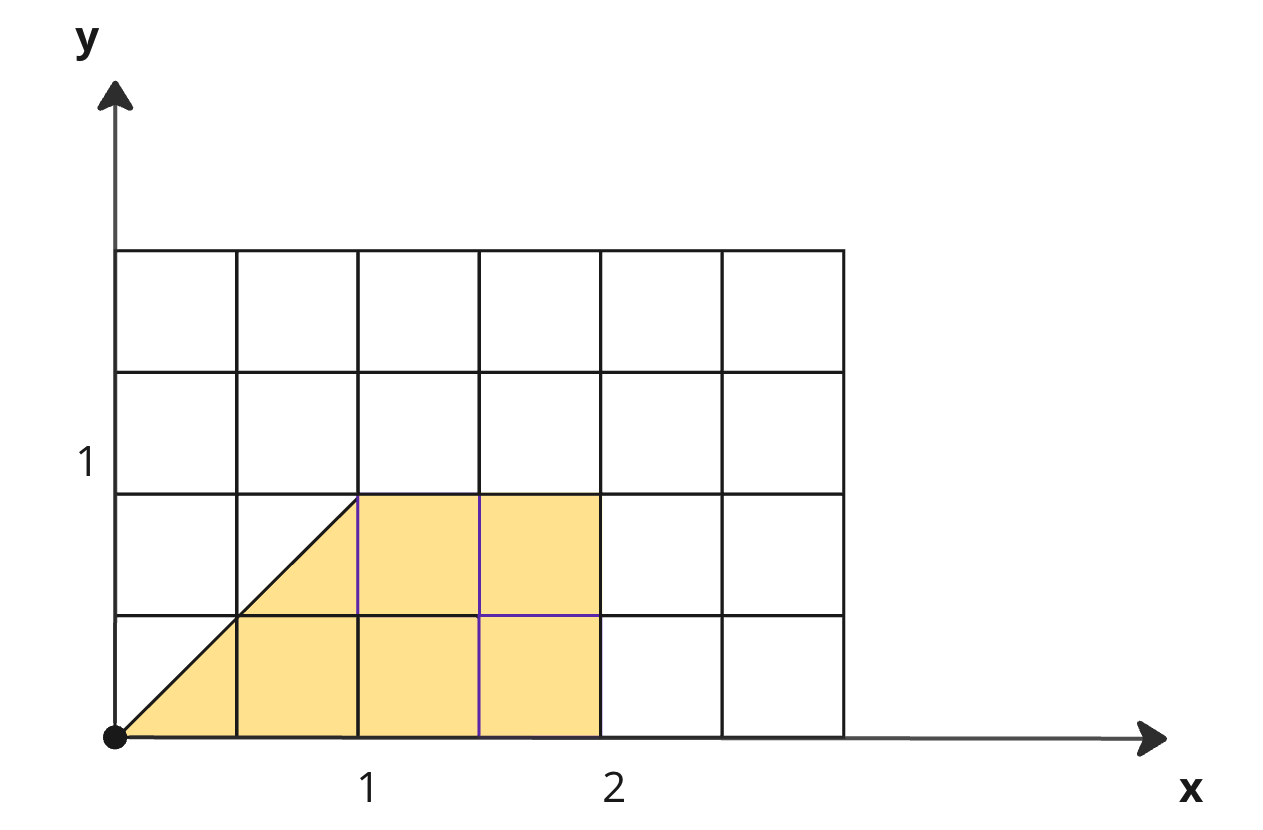
\includegraphics[width=0.7\textwidth]{q7}
        \end{figure} \\
        We calculate $P(Y \leq X)$ as follows
        \begin{align*}
            P(Y \leq X) & = \int_{0}^{1} \int_{y}^{2} f(x, y)\; dx dy                                                                                              \\
                        & = \int_{0}^{1} \int_{y}^{2} \left(\frac{1}{2}\right)x^2y + \left(\frac{1}{3}\right)y\; dx dy                                             \\
                        & = \int_{0}^{1} \left(\frac{1}{6}\right)x^3y + \left(\frac{1}{3}\right)xy \Big|_y^2\; dy                                                  \\
                        & = \int_{0}^{1} \left(\frac{4}{3}\right)y + \left(\frac{2}{3}\right)y - \left(\frac{1}{6}\right)y^4 - \frac{1}{3}y^2\; dy                 \\
                        & = \left(\frac{2}{3}\right)y^2 + \left(\frac{1}{3}\right)y^2 - \left(\frac{1}{30}\right)y^5 - \left(\frac{1}{9}\right)y^3 \Big|_0^1 \; dy \\
                        & = \left(\frac{2}{3}\right) + \left(\frac{1}{3}\right) - \left(\frac{1}{30}\right) - \left(\frac{1}{9}\right)                             \\
                        & = \boldsymbol{\frac{77}{90}}
        \end{align*}
        %%%%%%%%%%%%%%%%%%%%%%%%%%%%%%%%%%%%%%%%%%%%%%%%%%%%%%%%%%%%%%%%%%%%%%%%%%%%%%%%%%%%%%%%%%%%%%%%%%%%       
        %%%%%%%%%%%%%%%%%%%%%%%%%%%%%%%%%%%%%%%%%%%%%%%%%%%%%%%%%%%%%%%%%%%%%%%%%%%%%%%%%%%%%%%%%%%%%%%%%%%%       
        %%%%%%%%%%%%%%%%%%%%%%%%%%%%%%%%%%%%%%%%%%%%%%%%%%%%%%%%%%%%%%%%%%%%%%%%%%%%%%%%%%%%%%%%%%%%%%%%%%%%            
        \textbf{Question 8} \\
        A box contains two red, three green, and five blue chips. Two chips are selected from the box.
        Let $X_1$ and $X_2$ denote the number of red and green chips obtained.
        \begin{enumerate}
            \item Find the probabilities associated with all possible pairs of values $(x_1,
                      x_2)$.
            \item Determine the marginal probabilities associated with $X_1, X_2$.
            \item Determine the $f_{X_2}(x_2 = 1 | x_1 = 0)$.
        \end{enumerate}
        \textbf{Solution}
        \begin{enumerate}
            \item The probabilties associate with a pair of $(x_1, x_2)$ can be calculated as
                  follows
                  \begin{align*}
                      P(X_1 = x_1, X_2 = x_2) & = \frac{\binom{2}{x_1}\binom{3}{x_2}\binom{5}{5-x_1-x_2}}{\binom{10}{2}}
                  \end{align*}
                  The probabilities associated with all possible pairs of values $(x_1, x_2)$ are
                  \begin{center}
                      \begin{tabular}{|c|c|c|c|}
                          \hline
                                  & $X_1=0$         & $X_1=1$         & $X_1=2$        \\
                          \hline
                                  &                 &                 &                \\
                          $X_2=0$ & $\frac{10}{45}$ & $\frac{10}{45}$ & $\frac{1}{45}$ \\
                                  &                 &                 &                \\
                          $X_2=1$ & $\frac{15}{45}$ & $\frac{6}{45}$  & 0              \\
                                  &                 &                 &                \\
                          $X_2=2$ & $\frac{3}{45}$  & 0               & 0              \\
                                  &                 &                 &                \\
                          \hline
                      \end{tabular}
                  \end{center}
            \item The marginal probabilities associated with $X_1$ and $X_2$ are
                  \begin{align*}
                      P(X_1 = 0) & = \frac{10}{45} + \frac{15}{45} + \frac{3}{45} = \boldsymbol{\frac{28}{45}} \\
                      P(X_1 = 1) & = \frac{10}{45} + \frac{6}{45} = \boldsymbol{\frac{16}{45}}                 \\
                      P(X_1 = 2) & = \boldsymbol{\frac{1}{45}}                                                 \\
                      P(X_2 = 0) & = \frac{10}{45} + \frac{10}{45} + \frac{1}{45} = \boldsymbol{\frac{21}{45}} \\
                      P(X_2 = 1) & = \frac{15}{45} + \frac{6}{45} = \boldsymbol{\frac{21}{45}}                 \\
                      P(X_2 = 2) & = \boldsymbol{\frac{3}{45}}
                  \end{align*}
            \item The conditional probability $f_{X_2}(x_2 = 1 | x_1 = 0)$ is calculated as
                  follows
                  \begin{align*}
                      f_{X_2}(x_2 = 1 | x_1 = 0) & = \frac{P(X_1 = 0, X_2 = 1)}{P(X_1 = 0)} \\
                                                 & = \frac{\frac{15}{45}}{\frac{28}{45}}    \\
                                                 & = \boldsymbol{\frac{15}{28}}
                  \end{align*}
        \end{enumerate}
        %%%%%%%%%%%%%%%%%%%%%%%%%%%%%%%%%%%%%%%%%%%%%%%%%%%%%%%%%%%%%%%%%%%%%%%%%%%%%%%%%%%%%%%%%%%%%%%%%%%%       
        %%%%%%%%%%%%%%%%%%%%%%%%%%%%%%%%%%%%%%%%%%%%%%%%%%%%%%%%%%%%%%%%%%%%%%%%%%%%%%%%%%%%%%%%%%%%%%%%%%%%       
        %%%%%%%%%%%%%%%%%%%%%%%%%%%%%%%%%%%%%%%%%%%%%%%%%%%%%%%%%%%%%%%%%%%%%%%%%%%%%%%%%%%%%%%%%%%%%%%%%%%%  
        \textbf{Question 9} \\
        In a gambling game, five fair coins are tossed. For a bet of \$5, a gambler will win \$10 if three
        heads occur. Otherwise, the gambler loses the \$5 bet. What is the expected gain for a typical
        bet of \$5.
        \textbf{Solution} \\
        Probability of winning \$10 is
        \begin{align*}
            P(\text{win}) & = \binom{5}{3} \left(\frac{1}{2}\right)^3 \left(\frac{1}{2}\right)^2 \\
                          & = \frac{5}{16}
        \end{align*}
        Probability of losing \$5 is
        \begin{align*}
            P(\text{lose}) & = 1 - P(\text{win}) \\
                           & = 1 - \frac{5}{16}  \\
                           & = \frac{11}{16}
        \end{align*}
        The expected gain for a typical bet of \$5 is
        \begin{align*}
            E(\text{gain}) & = 10 \times P(\text{win}) - 5 \times P(\text{lose}) \\
                           & = 10 \times \frac{5}{16} - 5 \times \frac{11}{16}   \\
                           & = \boldsymbol{-\frac{5}{16}}
        \end{align*}
        %%%%%%%%%%%%%%%%%%%%%%%%%%%%%%%%%%%%%%%%%%%%%%%%%%%%%%%%%%%%%%%%%%%%%%%%%%%%%%%%%%%%%%%%%%%%%%%%%%%%       
        %%%%%%%%%%%%%%%%%%%%%%%%%%%%%%%%%%%%%%%%%%%%%%%%%%%%%%%%%%%%%%%%%%%%%%%%%%%%%%%%%%%%%%%%%%%%%%%%%%%%       
        %%%%%%%%%%%%%%%%%%%%%%%%%%%%%%%%%%%%%%%%%%%%%%%%%%%%%%%%%%%%%%%%%%%%%%%%%%%%%%%%%%%%%%%%%%%%%%%%%%%%  
        \textbf{Question 10} \\
        In a certain country the heights for adult males are normally distributed with a mean of 68 inches
        and a standard deviation of 4 inches. Let X symbolize the height.
        \begin{enumerate}
            \item Determine the probability $P(66 < X < 73)$.
            \item Determine the height which represents the $90^{th}$ percentile.
        \end{enumerate}
        \textbf{Solution}
        \begin{enumerate}
            \item The probability $P(66 < X < 73)$ is
                  \begin{align*}
                      P(66 < X < 73) & = P\left(\infty < X \leq 73\right) - P\left(\infty < X \leq 66\right)     \\
                                     & = \Phi\left(\frac{73 - 68}{4}\right) - \Phi\left(\frac{66 - 68}{4}\right) \\
                                     & = \Phi(1.25) - \Phi(-0.5)                                                 \\
                                     & = 0.8944 - 0.3085                                                         \\
                                     & = \boldsymbol{0.5859}
                  \end{align*}
            \item The height which represents the $90^{th}$ percentile is
                  \begin{align*}
                      \Phi(z) & = 0.9               \\
                      z       & = \boldsymbol{1.28}
                  \end{align*}
                  The height which represents the $90^{th}$ percentile is
                  \begin{align*}
                      x & = 1.28 \times 4 + 68 \\
                        & = \boldsymbol{73.12}
                  \end{align*}
        \end{enumerate}
        %%%%%%%%%%%%%%%%%%%%%%%%%%%%%%%%%%%%%%%%%%%%%%%%%%%%%%%%%%%%%%%%%%%%%%%%%%%%%%%%%%%%%%%%%%%%%%%%%%%%       
        %%%%%%%%%%%%%%%%%%%%%%%%%%%%%%%%%%%%%%%%%%%%%%%%%%%%%%%%%%%%%%%%%%%%%%%%%%%%%%%%%%%%%%%%%%%%%%%%%%%%       
        %%%%%%%%%%%%%%%%%%%%%%%%%%%%%%%%%%%%%%%%%%%%%%%%%%%%%%%%%%%%%%%%%%%%%%%%%%%%%%%%%%%%%%%%%%%%%%%%%%%%  
        \textbf{Question 11} \\
        Given that $f(x) = ke^{-x/3}$ for $x > 0$, and $f(x) = 0$ elsewhere.
        \begin{enumerate}
            \item Determine $k$.
            \item Determine the CDF of X.
        \end{enumerate}
        \textbf{Solution}
        \begin{enumerate}
            \item The value of $k$ is determined by
                  \begin{align*}
                      \int_{0}^{\infty} f(x)\; dx                & = 1                        \\
                      \int_{0}^{\infty} ke^{-x/3}\; dx           & = 1                        \\
                      k \int_{0}^{\infty} e^{-x/3}\; dx          & = 1                        \\
                      k \left(-3e^{-x/3}\right) \Big|_0^\infty   & = 1                        \\
                      k \left(-3e^{-\infty/3} + 3e^{-0/3}\right) & = 1                        \\
                      k \left(-3 \times 0 + 3 \times 1\right)    & = 1                        \\
                      k                                          & = \boldsymbol{\frac{1}{3}}
                  \end{align*}
            \item The CDF of $X$ is
                  \begin{align*}
                      F(x) & = \int_{0}^{x} f(x)\; dx                          \\
                           & = \int_{0}^{x} \frac{1}{3}e^{-x/3}\; dx           \\
                           & = \frac{1}{3} \int_{0}^{x} e^{-x/3}\; dx          \\
                           & = \frac{1}{3} \left(-3e^{-x/3}\right) \Big|_0^x   \\
                           & = \frac{1}{3} \left(-3e^{-x/3} + 3e^{-0/3}\right) \\
                           & = \boldsymbol{1 - e^{-x/3}}
                  \end{align*}
        \end{enumerate}
        %%%%%%%%%%%%%%%%%%%%%%%%%%%%%%%%%%%%%%%%%%%%%%%%%%%%%%%%%%%%%%%%%%%%%%%%%%%%%%%%%%%%%%%%%%%%%%%%%%%%       
        %%%%%%%%%%%%%%%%%%%%%%%%%%%%%%%%%%%%%%%%%%%%%%%%%%%%%%%%%%%%%%%%%%%%%%%%%%%%%%%%%%%%%%%%%%%%%%%%%%%%       
        %%%%%%%%%%%%%%%%%%%%%%%%%%%%%%%%%%%%%%%%%%%%%%%%%%%%%%%%%%%%%%%%%%%%%%%%%%%%%%%%%%%%%%%%%%%%%%%%%%%%  
        \textbf{Bonus Question} \\
        Derive Bayes Theorem given in Theorem 2.4.2 on page 45. \\
        \begin{align*}
            P(A_j | B) & = \frac{P(B | A_j) P(A_j)}{\sum_{i=1}^{n} P(B | A_i) P(A_i)}
        \end{align*}
        \textbf{Solution} \\
        Refer to the Definition 2.4.1 of conditional probability, we have the following
        \begin{align*}
            P(A_j | B) & = \frac{P(A_j \cap B)}{P(B)}                \\
                       & = \frac{P(B | A_j) P(A_j)}{P(B)} \qquad (1)
        \end{align*}
        Refer to the Theorem 2.4.1 of the law of total probability, we have the following
        \begin{align*}
            P(B) & = \sum_{i=1}^{n} P(B | A_i) P(A_i) \qquad (2)
        \end{align*}
        From (1), (2), we derives Bayes Theorem in Theorem 2.4.2 as follows
        \begin{align*}
            P(A_j | B) & = \frac{P(B | A_j) P(A_j)}{\sum_{i=1}^{n} P(B | A_i) P(A_i)}
        \end{align*}
        %%%%%%%%%%%%%%%%%%%%%%%%%%%%%%%%%%%%%%%%%%%%%%%%%%%%%%%%%%%%%%%%%%%%%%%%%%%%%%%%%%%%%%%%%%%%%%%%%%%%         
        %%%%%%%%%%%%%%%%%%%%%%%%%%%%%%%%%%%%%%%%%%%%%%%%%%%%%%%%%%%%%%%%%%%%%%%%%%%%%%%%%%%%%%%%%%%%%%%%%%%%         
        %%%%%%%%%%%%%%%%%%%%%%%%%%%%%%%%%%%%%%%%%%%%%%%%%%%%%%%%%%%%%%%%%%%%%%%%%%%%%%%%%%%%%%%%%%%%%%%%%%%%         
        %%%%%%%%%%%%%%%%%%%%%%%%%%%%%%%%%%%%%%%%%%%%%%%%%%%%%%%%%%%%%%%%%%%%%%%%%%%%%%%%%%%%%%%%%%%%%%%%%%%%         
        %%%%%%%%%%%%%%%%%%%%%%%%%%%%%%%%%%%%%%%%%%%%%%%%%%%%%%%%%%%%%%%%%%%%%%%%%%%%%%%%%%%%%%%%%%%%%%%%%%%%                 
\end{enumerate}
%%%%%%%%%%%%%%%%%%%%%%%%%%%%%%%%%%%%%%%%%%%%%%%%%%%%%%%%%%%%%%%%%%%%%%%%%%%%%%%%%%%%%%%%%%%%%%%%%%%%    
\end{document}